\section{Ingestion module for the REP\_OPDPC file}

This sections describes the ingestion module for inserting the \acrshort{dpc} processing analysis.

The associated ingestion processor is:

\begin{itemize} 

\item \textbf{s2boa.ingestions.ingestion\_dpc.ingestion\_dpc}
  
\end{itemize}

This module uses the following \acrshort{dim} signatures:

\begin{itemize} 

\item \textbf{PROCESSING\_XXX}: data corresponding to the processing analysis.

\item \textbf{COMPLETENESS\_NPPF\_XXX}: data corresponding to the definition of planning completeness used for analysis.

\item \textbf{ISP\_VALIDITY\_PROCESSING\_COMPLETENESS\_XXX}: data corresponding to the definition of \acrshort{isp} processing completeness used for analysis.

\item \textbf{INDEXING\_XXX}: data corresponding to the indexing analysis of products.

\item \textbf{ARCHIVING}: data corresponding to the archiving analysis of products.

\item \textbf{CATALOGING}: data corresponding to the cataloging analysis of products.

\item \textbf{LONG\_TERM\_ARCHIVING}: data corresponding to the cataloging analysis of products.

\end{itemize}

Where XXX is the corresponding satellite id.

The figure \ref{fg:structure_ingestion_dpc} shows a simplified diagram of the structure of events inserted (associated structure of values not included for simplicity).

\begin{figure}[H]
  \begin{center}
	\centering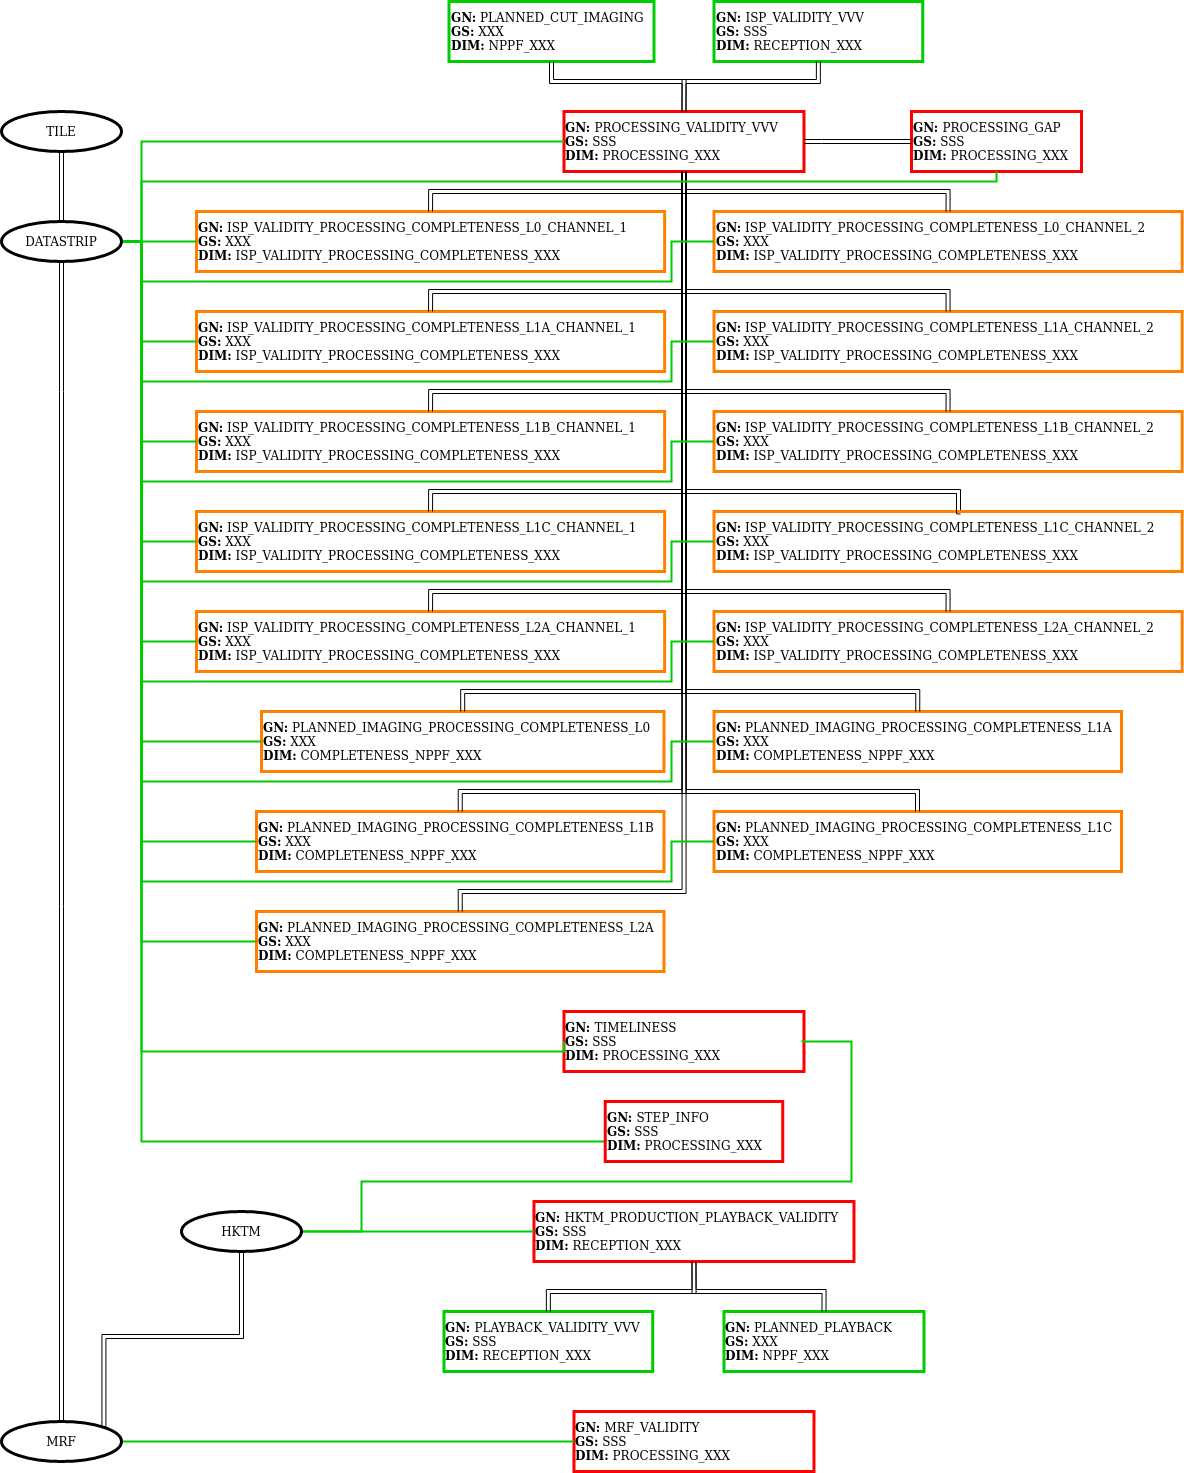
\includegraphics[width=150mm]{../fig/structure_ingestion_dpc.png}
	\caption{Structure of events inserted by the ingestion module for the REP\_OPDPC file}
	\label{fg:structure_ingestion_dpc}
  \end{center}
\end{figure}

The table \ref{tb:description_events_ingestion_dpc} shows the description of the events inserted by the ingestion.

